\chapter{Literature Review, Contributions and Scope} 

\label{chap:lit_review} 

\lhead{Chapter 2. \emph{Literature Review, Contributions and Scope}} 

The aim of this literature review is to provide an overview of the field of Graph Signal Processing (GSP) with a particular emphasis on multivariate reconstruction and regression models. First, we will give some historical context for the subject, highlighting the key theoretical advancements and canonical examples, before moving towards the contemporary developments relevant to this thesis. This begins with a discussion of graph filters and kernels, which are a fundamental building block of the methods presented in this thesis. Next, we discuss the topic of graph signal reconstruction, before covering different approaches to regression with graph signals. This is followed by a survey the emerging field of multiway graph signal processing, and finally we discuss node classification methods. For each of this topics we explain how the methods presented in this thesis contribute to the field. 

By presenting a holistic view of the existing literature, this review aims to set a firm foundation upon which we can build the discussion for our ensuing research questions. In addition, this chapter will also hone in on the specific scope of this thesis and define the boundaries of our research. In particular, we aim to identify the areas of interest that remain under-explored or incomplete in the current state of research, as well as clearly demarcate the topics which are not directly relevant to our research focus. 


\section{A historical perspective on GSP}

Though GSP as a field in its own right is generally understood to have been established in the early 2000s, its underlying conceptual framework draws upon the well-established fields of Spectral Graph Theory (SGT), and Digital Signal Processing (DSP), which both date back several decades. SGT is a branch of mathematics that studies the eigenvalues and eigenvectors associated with a graph's adjacency or Laplacian matrix to gain insight into its structural properties \citep{Chung1997}. Early work on SGT can be traced back to the 1950s and '60s \citep{Collatz1957,Hoffman1969}, although many of the concepts had already been studied in parallel within quantum chemistry \citep{Huckel1931}. One of the foundational results in SGT is the multiplicity of the Laplacian's zero eigenvalue gives the number of connected components in the graph \citep{Cvetkovic1980}. Another key result is Cheeger's inequality, which relates the second smallest eigenvalue of the Laplacian (also known as the algebraic connectivity) to the isoperimetric number of the graph (a measure of a graph's bottleneck) \citep{Cheeger1971}. 

Digital Signal Processing (DSP), sometimes considered a branch of engineering, utilises digital computation to analyse, transform, or filter signals, which can be in forms such as sound, images, and sensor data \citep{Rabiner1975}. The core principles of DSP are grounded in linear algebra, calculus, differential equations, and statistics. This theoretical underpinning has led to a plethora of practical applications across varied fields, such as telecommunications, audio processing, image and video processing, astronomy, and seismology, to name a few. Within DSP, the Discrete Fourier Transform (DFT) and its fast algorithmic implementation, the Fast Fourier Transform (FFT), play a central role, with many tasks such as reconstruction, denoising, compression, and filtering requiring analysis and manipulation of the frequency content of signals \citep{Duhamel1990}.

GSP began to take shape as a separate discipline around the start of the 21st century, as the proliferation of data and advancements in computer technology gave rise to more complex, irregular, and high-dimensional data structures. The theoretical framework underpinning GSP emerged from work on Algebraic Signal Processing (ASP), with several papers published by Puschel and Moura from 2003 to 2008 establishing an axiomatic approach to discrete time signal processing \citep{Puschel2003,Puschel2006,Puschel2008}. This mathematical formalism, based on the concept of shift operators, established a unifying framework for several concepts from classical signal processing. For example, under the ASP paradigm, the Discrete Cosine Transform (DCT) and DFT are understood as generated from different discrete shift operators (a chain and cycle respectively) \citep{Isufi2022}. 

Meanwhile, in the data science and machine learning community, concepts from SGT were being applied to nonlinear dimensionality reduction using the Laplacian eigenbasis \citep{Roweis2000,Belkin2003,Donoho2003}. This was followed by work such as \cite{Kondor2002}
and \cite{Smola2003}, who studied the topic of graph kernels. This work was subsequently applied in semi-supervised learning, where the goal is to maximise the utility of unlabelled data using its topology in feature space \citep{Belkin2004,Zhou2004,Zhu2003}. We return to the topic of graph kernels in greater detail in \cref{sec:graph_kernels}. 

Around the same time, in the signal processing community, authors were working on both distributed and global algorithms for denoising and regression on sensor networks \cite{Guestrin2004,Wagner2005,Wagner2006}. 

In the early 2010s, two distinct yet complementary approaches to GSP emerged, as discussed in \cite{Leus2023}. The first approach, often credited to \cite{Sandryhaila2013,Sandryhaila2013b}, adopted an algebraic perspective, building upon existing work in Algebraic Signal Processing. This methodology primarily focused on defining the Graph Fourier Transform and related concepts using the foundational operation of graph shifts. Conversely, the second approach, as proposed by  \cite{Hammond2011,Shuman2013}, endorsed the use of the graph Laplacian as the core component for GSP algorithms. This second paradigm, which aligns closely with the concepts presented in \cref{sec:fundamentals}, is also the primary approach utilised in this thesis.


\section{Graph kernels and graph filters}

\label{sec:graph_kernels}

In GSP, two distinct but closely-related concepts are graph filters and graph kernels. In the Laplacian-based GSP paradigm, both can understood as a function $g(\lambda)$ applied to the frequency profile of a graph signal or, equivalently, a power series applied to the Laplacian itself. Note that, in this context, graph kernel should not be confused with another concept that bares the same name which refers to distance measures between pairs of graphs \citep{Kriege2020}. Graph filters and graph kernels provide a map $\R^N \mapsto \R^N$, and can be represented as a matrix operator $\HH \in \R^{N \times N}$.

\begin{equation}
    \HH = g(\LL) = \U g(\LAM) \U^\top
\end{equation}

 $g(\cdot)$ can be set such that it promotes certain properties in the output signal, for example, a low-pass filter (such as those specified in \cref{tab:filters}) is monotonically decreasing function which attenuates the high frequency content of a signal. In the GSP community, typically the terms `filter' is preferred to refer to this class of operator \citep{Shuman2013}, however, there are those who prefer the term `kernel' \citep{Ioannidis2016,Romero2017}. Often the difference is simply that a kernel is an increasing function, used to construct penalty terms, whereas a filter is a decreasing one, used to operate on graph signals. In the machine learning community, the term kernel is typically preferred \cite{Kondor2002,Smola2003}. Either convention can be used, and in this thesis we use filters for the most part. 


\subsection{Probability distributions over graph signals}

Spectral operators can be used to define probability distributions over smooth graph signals. An early example of this is found in \cite{Gadde2015}, where the authors propose a Gaussian Random Field (GRF) model for the generation of graph signals. In particular, they build a model for vertex sampling that assumes signals are random variables drawn from the following underlying multivariate Gaussian distribution. 


\begin{equation}
    \y \sim \Norm{\zero}{(\LL + \delta \I)^{-1}}
\end{equation}


This probabilistic interpretation offers a principled way of reasoning about graph signals, making the relationship between GSP and certain methods from semi-supervised learning more apparent \citep{Zhu2003}. More recently, in \cite{Venkitaraman2020}, the authors propose using graph filters to specify a probability distribution. In particular, they advocate using the following Gaussian distribution. 

\begin{equation}
    \label{eq:gaussian_filter}
    \y \sim \Norm{\zero}{\gamma^{-1} \HH^2}
\end{equation}

\begin{wrapfigure}{r}{0.4\linewidth}
	\centering
		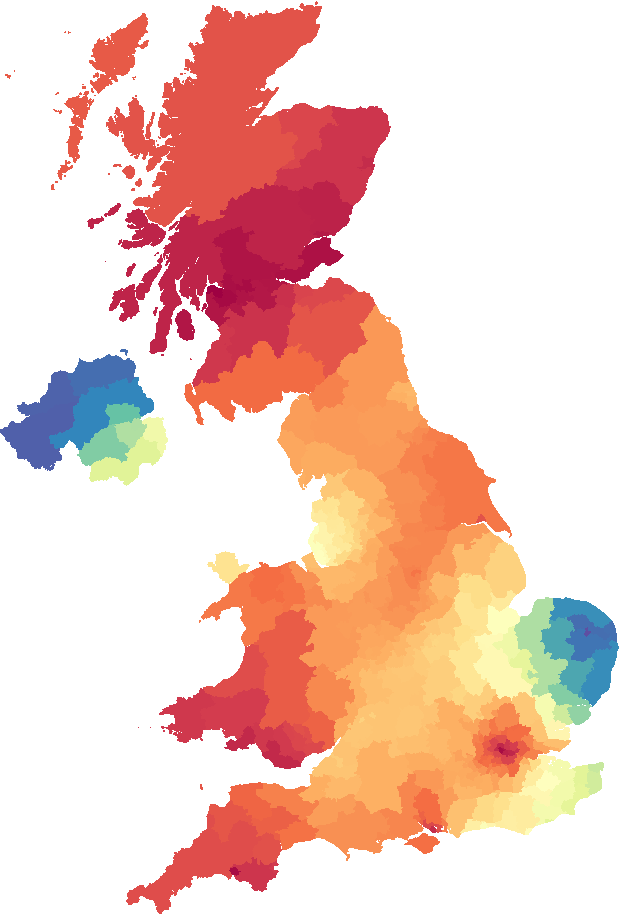
\includegraphics[width=0.7\linewidth]{Figures/uk_smooth.pdf}
	\caption[An example of a random smooth graph signal]{An example of a random smooth signal on the UK district graph, sampled from $\Norm{\zero}{\HH^2}$ using a bandlimited filter. }
	\label{fig:random_smooth_uk}
\end{wrapfigure}

where $\HH$ is a generic graph filter. The justification for this is as follows. Consider an independent multivariate normal random variable $\y \sim \Norm{\zero}{\I_N}$. Applying a graph filter to a random signal $\x$ will result in a new signal, $\HH \x$, which is smoother with respect to the graph topology. This will be distributed according to $\HH \x \sim \Norm{\zero}{\HH^2}$, meaning $\HH^2$ can be interpreted as a covariance matrix with which to generate smooth, normally distributed graph signals. This more flexible approach allows for various beliefs about the frequency profile of graph signals to be encoded. \Cref{fig:random_smooth_uk} shows an example of a random signal drawn from the distribution of \cref{eq:gaussian_filter}. 

In a similar manner, \citep{Perraudin2017} suggest a flexible class of Laplacian-based covariance matrices, although this approach lacks the interpretability of the aforementioned filter-based formulation. In this thesis, we follow the example of \cite{Venkitaraman2020}, extending their method to describe distributions over multidimensional graph signals (two-dimensional matrix signals in \cref{chap:gsr_2d}, and $d$-dimensional tensor signals in \cref{chap:nd_gsp}). This allows us to build a rich class of Bayesian models for tasks such as reconstruction and regression. 

\subsection{Approximating graph filters with Chebyshev polynomials}

\label{sec:Chebyshev}

A popular and longstanding technique, which can be traced back to some of the earliest work on Laplacian-based GSP \citep{Hammond2011}, involves computing the action of a graph filter using Chebyshev polynomials. These functions, which form an orthonormal basis on the space $L^2 \left([-1, 1], \frac{dx}{\sqrt{1 - x^2}}\right)$ \citep{Mason2002}, can be used to approximate an arbitrary graph filter function $h(\lambda)$. Since the domain of the filter is $[0, \lambda_{\text{max}}]$, first consider the change of variables $\lambda = \frac{1}{2}\lambda_{\text{max}}(x + 1)$ to define the shifted Chebyshev polynomials as follows. 

\begin{equation}
    \bar{T}_k(\lambda) := T_{k}\left(\frac{2\lambda - \lambda_{\text{max}}}{\lambda_{\text{max}}}\right)
\end{equation}

The target filter function is then expanded using $K$ terms as follows. 

\begin{figure}[t]
	\centering
		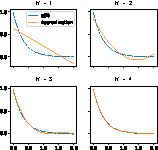
\includegraphics[width=0.7\linewidth]{Figures/cheb.pdf}
	\caption[Successive approximations of a filter function using Chebyshev polynomials.]{Successive approximations of the filter function $g(\lambda) = \exp(-3\lambda)$ using Chebyshev polynomials. }
	\label{fig:Chebyshev}
\end{figure}


\begin{equation}
    h(\lambda) \approx \sum_{k=0}^K c_k \bar{T}_k(\lambda)
\end{equation}

The coefficients, $c_k$, are given by the solution to the following integral and can be quickly computed numerically. 

\begin{equation}
    \label{eq:Cheb_int}
    c_k = \begin{cases}
        \displaystyle   
        \; \frac{1}{\pi} \int_{0}^{\pi} h\left(\frac{\lambda_{\text{max}}}{2} (\cos(\theta) + 1)\right) \, d\theta & \text{if} \quad k = 0, \\[0.8cm]
        \displaystyle   
        \; \frac{2}{\pi} \int_{0}^{\pi} \cos(k \theta) \; h\left(\frac{\lambda_{\text{max}}}{2} (\cos(\theta) + 1)\right) \, d\theta & \text{otherwise.}
    \end{cases}
\end{equation}

The benefit of this approach is that Chebyshev polynomials can be defined recursively as follows. 

\begin{equation}
    \bar{T}_k(\lambda) = \left(\frac{4 \lambda }{\lambda_{\text{max}}}  - 2\right) \bar{T}_{k-1}(\lambda) - \bar{T}_{k-2}(\lambda)
\end{equation}

with the initial values

\begin{equation}
    \bar{T}_0 = 1, \quad \bar{T}_1 = \frac{2 \lambda }{\lambda_{\text{max}}} - 1
\end{equation}

This means that the computation can be applied in a distributed manner using message passing, or simply that computationally expensive eigenvalue decomposition of the Laplacian can be avoided \citep{Shuman2018}. In particular, if the Laplacian is sparse (which is often the case), its action onto a vector can be computed with complexity proportional to the number of edges. 


\section{Graph Signal Reconstruction}

Graph Signal Reconstruction (GSR), sometimes also known as graph signal interpolation, is a classic problem in GSP \citep{Ortega2018}. The task can be stated as, given a partially observed graph signal, estimate the signal value at the unobserved vertices using only the topology of the graph. Closely related, is the topic of signal sampling, which seeks to find an informative set of vertices to measure a graph signal at, in order to perform an accurate reconstruction \citep{Tanaka2020}. Typically, GSR is posed as an optimisation problem where one seeks to identify a smooth underlying graph signal that simultaneously minimises a measure of error across the observed nodes, as well as a penalty term that enforces some kind of signal smoothness or bandlimited assumption. 

Early work on GSR, such as \cite{Narang2013b,Narang2013,Wang2015b,Anis2016}, mainly focused on the reconstruction of bandlimited graph signals. Here, the goal is to find the optimal reconstruction of a signal using only the first $K$ eigenvectors of the graph Laplacian, with a frequency less than $\omega$ (the so-called Paley-Wiener space). In \cite{Narang2013b}, this is achieved using an Iteratively Reweighted Least Squares (IRLS) algorithm, with a Chebyshev polynomial approximation to the bandlimited filter. Further work such as \citep{Romero2017b} proposes using a more flexible specification of the reconstructed signal profile based on graph kernels. 

Several methods have also been proposed for the reconstruction of time-varying graph signals. In \cite{Qiu2017}, the penalty term in the optimisation objective promotes both smoothness across the graph using a Laplacian penalty, and consistency across time, by introducing a temporal difference operator $\D$. The problem is then solved for both the noiseless and noisy case using a gradient projection algorithm with backtracking line search. A similar method is adopted in \cite{Giraldo2022}, but with a regularised version of the Laplacian for improved computational robustness. In \cite{Ioannidis2016}, this approach is modified to incorporate a more dynamic penalty that can adjust the strength of regularisation across the graph and across time independently, using so-termed ``space-time kernels''. Furthermore, in this paper, as well as \cite{Romero2017,Ioannidis2018}, the authors propose an online algorithm that can accommodate dynamic graphs (i.e. graphs for which the edge weights can change over time), although this is only possible for a special class of kernel which have a tri-diagonal inverse. 

Recently, some methods have also been proposed for distributed reconstruction of time varying graph signals. In \cite{Chi2022}, as well as \citep{Zhou2022b}, the authors propose distributed algorithms that draw upon the work of \cite{Qiu2017} using the temporal difference operator. In these two papers, which have similar goals but were developed separately, the authors use a modified Newton method to solve the optimisation problem, by making use of an approximation to the Hessian. 

In this thesis, we take inspiration from space-time kernels developed in \cite{Ioannidis2016}, as well as the graph spectral priors of \cite{Venkitaraman2020}, to develop a flexible Bayesian formulation of the reconstruction problem. In addition, while the problem of time-varying graph signal reconstruction has been examined by several papers, in \cref{chap:gsr_2d} we propose reconstruction on two-dimensional Cartesian products graphs, of which time varying graph signals can be considered a special case. Furthermore, we offer two alternative optimisation algorithms, one a Stationary Iterative Method (SIM) using matrix splitting, and the other based on the Conjugate Gradient Method (CGM) with a specialised graph-spectral preconditioner. By conducting a detailed asymptotic analysis, we compare and contrast the convergence behaviour of these two algorithms. Whilst convergence is discussed in many of the aforementioned papers, we provide fresh insight into the effect of the model hyperparameters, and present synthetic data studies to confirm our theoretical findings. Furthermore, we show how the SIM can be conducted in a distributed manner, and how the fraction of missing data in the original graph signal affects which of these two methods is preferable. In \cref{chap:nd_gsp}, we extend our methods to encompass GSR on Cartesian products graphs with an arbitrary number of dimensions, under the multiway GSP paradigm. To the best of our knowledge, these all represent novel contributions to the field. 


\section{Graph Signal Regression}

Another key topic that runs through this thesis is graph signal regression. One of the earliest papers to reference regression in the context of GSP is \cite{Guestrin2004}. Here, the authors propose a distributed algorithm for computing a function that approximates a time-varying graph signal, with applications aimed specifically at sensor networks. This paper, which predates much of the work on Laplacian-based GSP, is primarily focused on efficient algorithms for communication between sensors, and in modern parlance is more akin to graph signal compression, as the authors seek a low-dimensional representation of the original signal. In can also be considered a particular class of distributed spatial regression, as they consider the $x$-$y$ coordinates of each sensor, rather than modelling the network in terms of nodes and edges. 

In this thesis, the definition of graph signal regression we use differs somewhat from this formulation. For our purposes, we consider graph signal regression to be the task of estimating a graph signal as a function of additional explanatory variables. In particular, we highlight two different scenarios which we term exogenous (global) and endogenous (local) regression. For the exogenous case, we examine work on Kernel Graph Regression (KGR) \citep{Venkitaraman2019} and related variants such as Gaussian Process on Graphs (GPoG) \cite{Venkitaraman2020}. For the endogenous case, we examine work on Regression with Network Cohesion (RNC) \citep{Li2019}. 


\subsection{Exogenous case: Kernel Graph Regression and Gaussian Processes on Graphs}

The task of graph regression with endogenous explanatory variables can be stated as follows. Consider a series of $T$ real-valued graph signals, each measured on a graph comprising $N$ nodes, $\{\y_t \in \R^N\}_{t=1}^T$. Each of these signals has a corresponding associated length-$M$ vector of explanatory variables $\{\x_t\}_{t=1}^T$. The goal is to learn a function that maps the explanatory variables to the graph signals, such that if a new explanatory vector $\x'$ is supplied, we should be able to make an estimate for the corresponding graph signal $\y'$. By penalising predictions that are not smooth with respect to the topology of the graph, the intention is to produce an estimator that outperforms non graph-aware alternatives. Note that, while we use the index $t$ to denote each sample, the set $\{\x_t, \y_t\}$ can simply be regarded as training pairs and need not represent time-series data (although they often may). 


In this context, the variables are `exogenous' or global in the sense that they are not associated with any node in particular, and the signal at each node in the graph can learn a unique functional response. For example, consider a time-varying graph signal consisting of net profits for a network of businesses connected based on industry or supply chain. In this case, the explanatory variables could be factors in the broader economy such as GDP growth, inflation or unemployment which may affect each company differently. 

In \cite{Venkitaraman2019}, the authors propose Kernel Graph Regression (KGR) for this purpose. Here, each node in the observed graph signal $\y_t$ is modelled as a unique linear combination of a basis function representation of the explanatory variables $\boldsymbol{\phi}(\x_t) \in \R^P$, such that $\y_t = \W^\top \boldsymbol{\phi}(\x_t)$, where $\W \in \R^{P \times N}$ is a matrix of coefficients. To find the optimal value of $\W$, they propose the following cost function. 

\begin{equation}
    C(\W) = \sum_{t=1}^T ||\y_t - \W^\top \boldsymbol{\phi}(\x_t) ||_2^2 + \alpha \tr{\W^\top \W} + \beta \sum_{t=1}^T \text{TV}_2\big(\W^\top \boldsymbol{\phi}(\x_t)\big)
\end{equation}

The first term in this objective seeks to minimise the square prediction error, the second provides regularisation for the coefficient matrix, and the third utilises  the total square variation, of \cref{eq:TSV2}, to promote signal smoothness. Next, the authors leverage the so-called `kernel trick' to transform this to a non-parametric regression problem. This is achieved by introducing a $T \times T$ kernel matrix $\K$, where $\K_{ij} = \kappa(\x_i, \x_j)$ \citep{Rasmussen2005}, which results in the following in-sample prediction. 

\begin{equation}
    \mat{\big(\I_N \otimes \K\big)\big(\I_N \otimes (\K + \alpha \I_T) + \beta \LL \otimes \K \big)^{-1} \vecc{\Y}}
\end{equation}

where $\Y \in \R^{T \times N}$ is the matrix formed by stacking each observed signals $\{\y_t\}$, $\vecc{\cdot}$ represents column-major vectorisation mapping $\R^{T \times N} \mapsto \R^{TN}$, and $\mat{\cdot}$ is the reverse operation $\R^{TN}\mapsto  \R^{T \times N}$. The result is the prediction made over the training samples $\{\x_t\}_{t=1}^T$. This can also be adjusted to make a prediction for an unseen explanatory variable $\x'$. Some recent extensions have been proposed to KGR such as \cite{Elias2022}, where the authors use an algorithm based on random Fourier features to improve computational robustness. 

In \cite{Venkitaraman2020}, the same authors propose a new model which takes a Bayesian perspective to define Gaussian Processes over Graphs (GPG). Here, a modified approach is used, where a graph-spectral prior is placed over the coefficient matrix to induce smoothness in the output signal. This results in not only a point estimate for the signal, but a multivariate Gaussian probability distribution with a mean and covariance. In particular, the authors define an online algorithm where the distribution over a signal at time $T+1$, given $\x_{T+1}$ is given by 

\begin{equation}
     \Norm{\muu = \D^\top \C_T^{-1}\,\vecc{\Y}}{\; \SIG = \F - \D^\top \C_T^{-1} \D}
\end{equation}

with

\begin{align}
    \C_T &= \HH^2 \otimes \K + \beta^{-1} \I_N \otimes \I_T \\[0.1cm]
    \D &= \HH^2 \otimes \big[\kappa(\x_1, \x_{T+1}), \, \kappa(\x_2, \x_{T+1}), \, ... \, ,\, \kappa(\x_N, \x_{T+1})\big]^\top \\[0.1cm]
    \F &= \kappa(\x_{T+1}, \x_{T+1}) \HH^2 + \beta^{-1} \I_N
\end{align}

Several papers have also proposed extensions to this model. For example, in \cite{Miao2022}, the authors present a modified algorithm that simultaneously learns the underlying graph structure. In \cite{Zhi2023}, the authors propose parametrising the filter function as a finite polynomial of the graph Laplacian, and simultaneously learn the polynomial coefficients, extending their earlier work in \cite{Pu2021}. 

In \cref{chap:kgr_rnc_2d}, we present a hybrid model that incorporates aspects of graph signal reconstruction, as well as Gaussian processes over graphs. In particular, we are interested in reconstructing time-varying partially observed graph signals when additional exogenous explanatory variables exist. Notably, all the models discussed in this subsection assume that readings across all vertices are available as inputs into the model. However, in many real-world applications, node-level data may be corrupted by equipment failure or difficult/expensive to reliably collect. Whilst one option may be to simply remove problematic nodes from the problem entirely, this can waste valuable data that may help in the estimation problem. In \cref{chap:nd_gsp}, we take this further by developing a model that is capable of reconstructing $d$-dimensional multiway graph signals with exogenous variables. To the best of our knowledge, none of these issues have been addressed in the available literature. 


\subsection{Endogenous case: Regression with Network Cohesion}

The second graph regression setting we wish to highlight is the case when endogenous variables exist to aid with the estimation process. Consider a single graph signal $\y \in \R^N$, with elements existing on the nodes of a known graph. In this scenario, each node, $n$, has an associated vector of explanatory variables $\x_n \in \R^M$. The goal is to build a predictive model which utilised these local explanatory variables, whilst also incorporating the underlying structure of the network. 

In \cite{Li2019}, the authors propose Regression with Network Cohesion (RNC). Here, they propose modelling each element of the observed graph signal $\y_n$ as a linear combination of an intercept term and the explanatory variables at node $n$. This is summarised by the following statistical model. 

\begin{equation}
    \y = \cc + \X \w + \boldsymbol{\epsilon}
\end{equation}

$\X \in \R^{N \times M}$ is the matrix formed by stacking each vector of explanatory variables, $\w \in \R^M$ is a coefficient vector, and $\cc \in \R^N$ is a flexible intercept term of individual node effects. The model error $\boldsymbol{\epsilon} \in \R^N$ is assumed to have a zero mean and a variance of $\sigma^2 \I_N$. The model seeks to learn an optimal value for $\cc$ and $\w$ by minimising the following objective function. 

\begin{equation}
    \label{eq:RNC_objective}
    C(\cc, \w) = ||\y - \X \w - \cc ||^2_2 + \lambda \text{TV}_2(\cc)
\end{equation}

The addition of the total square variation term, which the authors name the cohesion penalty, is intended to promote smoothness over the flexible intercept with respect to the topology of the graph. The justification for this is that closely connected nodes are likely to have similar baseline effects, meaning the model simultaneously learns a shared coefficient vector $\w$, and a unique but smooth intercept. The optimal values can be computed by introducing a combined parameter vector $\thetaa = \begin{bmatrix} \cc \\ \w  \end{bmatrix}$, with an estimator given by 

\begin{equation}
    \label{eq:theta_RNC_OG}
    \hat{\thetaa} = \begin{bmatrix}
        \I_N + \lambda \LL & \X \\ \X^\top & \X^\top \X
    \end{bmatrix}^{-1} \begin{bmatrix}
        \I_N & \X
    \end{bmatrix} \y
\end{equation}

In order to make a prediction on a test set, where the new explanatory variables $\X' \in \R^{N' \times M}$ are available, the authors use the following. 

\begin{equation}
    \hat{\y}' = \hat{\cc}' + \X' \hat{\w}
\end{equation}

where $\hat{\w}$ is the optimal value found by minimising \cref{eq:RNC_objective}, and $\hat{\cc}'$ is found by minimising the following objective. 

\begin{equation}
    \hat{\cc}' = \underset{\cc'}{\text{argmin}} \quad \begin{bmatrix}
        \hat{\cc} \\ \cc' 
    \end{bmatrix}^\top \begin{bmatrix}
        \LL_{11} & \LL_{12} \\ \LL_{12}^\top & \LL_{22}
    \end{bmatrix} \begin{bmatrix}
        \hat{\cc} \\ \cc' 
    \end{bmatrix} = - \LL_{22}^{-1} \LL_{12}^\top \hat{\cc}
\end{equation}

where the new Laplacian characterising the full graph containing all train and test nodes has been broken into blocks as shown. Note that as long as the two parts of the graph are mutually connected, the inverse of $\LL_{22}$ will exist. As noted by the authors, there may be some issues surrounding computational robustness within this model. In particular, the system matrix found in \cref{eq:theta_RNC_OG} may in general be singular. To overcome this the authors propose adding a small term $\gamma \I_N$ to the graph Laplacian, which fixes this issue. 

One limitation of the RNC model is that the total variation penalty, while simple and easy to interpret, lacks the flexibility to specify more generic expectations about the spectral profile of the observed graph signal. 

\cite{Le2022}



\section{GSP on higher order graphs}

Multiway data processing 

\cite{Smilde2004}
\cite{Kroonenberg2008}


\cite{Ji2019}

\cite{Cammoun2009}


\subsection{Multi-Layer Graph Signal Processing}

\cite{Zhang2022} describe M-GSP 

\cite{Zhang2018} extend M-GSP to multiple layers with different number of nodes by adding fake nodes in where they are missing from layers. 
 

\subsection{Multi-Way Graph Signal Processing}


\cite{Zhao2023}

\cite{Li2012}



\section{Graph signal classification}

\cite{Tran2020}

\cite{Sandryhaila2013a}

\citep{Ahmed2017}

No one has done it on multiway graphs. Limited regression models. No one using graph filters. 

in ML: \citep{Belkin2002}




\section{Related topics}

For the sake of clarity, in this section we give a high-level overview of some important sub-fields of GSP which are adjacent to the work in this thesis, but not directly relevant to the core subject matter. While not addressed directly in this thesis, some of these topics offer potentially useful avenues for extension of our work. 


\subsection{Graph learning}

When GSP was originally formulated, the graph of interest was typically assumed to be known a priori, with the subsequent methods following from the existence of this basic structure. In real-world applications, this can often be the case, for example, in a social, transport or citation network it is clear how objects should be connected given the nature of the problem. In other applications, for example in a protein-protein interactome, domain specific knowledge can be incorporated in a principled way to construct a graph \citep{Li2023}. In others, such as a sensor network, $k$-nearest neighbour, $\varepsilon$-ball, or permuted minimum spanning tree techniques can be used to construct a reasonable graph \citep{Qiao2018}. 

However, in other circumstances, it may not be so clear how to derive or construct a graph, and instead one must be learned from the data. An example of this may be the stock price returns of a network of companies. While it may be possible to construct a graph using information such as industry, supply chain, or strategic alliance \citep{Gao2021,Cheng2021}, this information may be difficult to gather or otherwise unavailable. Another approach would be simply to learn a graph directly from the returns data. In general, the graph learning problem can be formulated as, given a set of graph signals $\{\y_t \in \R^N\}_{t=1}^T$, find an appropriate sparse $N \times N$ adjacency matrix \citep{Dong2019}. From the perspective of GSP, it is assumed that these observations are generated from some network process, operating on a latent underlying graph structure. 

One of the oldest and simplest approaches, predating work on GSP, is so-called correlation networks. Here, a graph can be constructed by considering the pairwise correlation between the signal at nodes $i$ and $j$. For example, one approach is to set $\A_{ij} = 1$ if $\rho_{ij} > 0$ and zero otherwise \citep{Mateos2019}. While such approaches are simple and have an intuitive notion of pairwise interaction, correlations may be due to latent network effects rather than from direct pairwise influence. For example, two nodes may be interacting via a third node $k$, in which case it is more prudent to set $\A_{ik} = \A_{jk} = 1$, and $\A_{ij} = 0$. While there are techniques to overcome such confounding of variables (see, \cite{Kolaczyk2009}, section 7), in general this can be problematic from the perspective of graph learning. 

An alternative prominent technique is the Graphical Lasso (GL) \citep{Friedman2007}. The GL is a sparse penalised maximum likelihood estimator for the precision matrix $\PP$ (the inverse of the covariance matrix $\SIG$) of a multivariate Gaussian random variable. The estimated value of $\PP$ is given by 

\begin{equation}
    \hat{\PP} = \underset{\PP \succcurlyeq 0}{\text{argmin}} \left[\tr{\PP \hat{\SIG}} - \log \det \left(\PP\right) + \lambda \sum_{i\neq j} |\PP_{ij}|\right]
\end{equation}

where $\hat{\SIG}$ is the sample covariance, with the L\textsubscript{1} norm promoting sparsity in $\PP$. The graph Laplacian is then derived by assuming $\PP$ is a regularised version of $\LL$ \citep{Lake2010}. 

Other approaches favour more GSP-oriented estimation models by incorporating signal smoothness assumptions. For example, in \cite{Hu2015}, the authors propose learning thee Laplacian matrix directly by solving the following optimisation problem. 

\begin{equation}
    \begin{gathered}
        \hat{\LL} = \text{argmin} \left[ \tr{\Y^\top \LL \Y} - \beta ||\LL ||_F^2 \right], \\ \text{s.t.} \quad \tr{\LL} = N, \quad \LL \one = \zero, \quad \LL_{ij} = \LL_{ji} >0
    \end{gathered}
\end{equation}

where $\Y \in \R^{N \times T}$ is the matrix obtained by stacking each observed graph signal $\y_t$. This was modified slightly in \cite{Dong2016} by introducing a new matrix $\X$, of the same dimensions as $\Y$, meant to be a smooth approximation of $\Y$. Their optimisation objective was then given by 

\begin{equation}
    \begin{gathered}
        \hat{\LL}, \hat{\X} = \text{argmin} \left[ ||\X - \Y||_F^2 + \alpha \tr{\X^\top \LL \X} - \beta ||\LL ||_F^2 \right], \\ \text{s.t.} \quad \tr{\LL} = N, \quad \LL \one = \zero, \quad \LL_{ij} = \LL_{ji} > 0
    \end{gathered}
\end{equation}

A more computationally efficient approach was proposed in \cite{Kalofolias2016}, but using the adjacency matrix rather than the Laplacian. There has been a substantial amount of additional work on graph learning from a GSP perspective. For a detailed review, see \cite{Dong2019,Mateos2019}. 


\subsection{GSP on directed graphs}

The work presented in this thesis, and indeed the majority of published literature on GSP, is focused on undirected graphs. The benefit of this framework is that the undirected graph Laplacian naturally gives rise to a simple definition of signal smoothness. It is also a well-behaved Hermitian operator, with real eigenvalues and orthonormal eigenvectors that serve as a well-motivated and coherent Fourier basis \citep{Ortega2018}. However, there is also a rich literature regarding GSP for directed graphs (or digraphs) \citep{Marques2020}. Directed graphs, while less commonly found in GSP, are more suitable for modelling certain applications such as web links, citation networks, trade flows and follower-model social networks, since they can accommodate both incoming and outgoing edges. However, extending the Graph Fourier Transform framework to signals on digraphs less straightforward and a number of alternative proposals exist. 

One originates from some of the earliest work on GSP from Sandryhaila and Moura, where the GFT for a general directed graph is constructed from the total variation of a graph signal $\y$ defined as follows. 

\begin{equation}
    \text{TV}_1(\y) = || \y - \A^{\text{norm}} \, \y ||_1
\end{equation}

where $\A^{\text{norm}}$ is the adjacency matrix (or, more generally, any graph shift operator) divided by its spectral radius to ensure that the transformed signal is appropriately scaled for comparison with the original signal \citep{Sandryhaila2013b}. A Fourier basis $\{\uu_i \}$ is then defined by first taking an eigendecomposition of the adjacency matrix, and then ordering the eigenvectors according to their total variation. Where the adjacency matrix is non-diagonalisable, one can instead resort to the generalised eigenvectors using Jordan decomposition. 

While this definition is attractive from a theoretical standpoint, it suffers from several drawbacks. In general, the eigenvectors are complex-valued and may be more difficult to interpret, for example, constant signals no longer have zero variation. Furthermore, the eigenvectors are typically non-orthonormal, meaning Parseval's identity no longer holds and  signal power is not preserved when transforming between the vertex and spectral domains. Other work has attempted to remedy this by proposing a new definition for variation on directed graphs. In \cite{Sardellitti2017}, the authors define the Graph Directed Variation (GDV) as follows. 

\begin{equation}
    \text{GDV}(\y) = \sum_{i,j}^N \A_{ij} [\y_i - \y_j]_{+}
\end{equation}

where $[\y_i - \y_j]_{+} = \text{max}(\y_i - \y_j, \, 0)$. The search for the GFT basis is then given by the optimisation problem of finding the set of orthonormal vectors that subsequently minimise the GDV subject to perpendicularity with all those preceding. Under this framework, smooth signals on digraphs represent a flow from a smaller value to a larger one over a directed edge. Hence, the signal at two nodes $i$ and $j$ is only penalised if $\y_i > \y_j$. For example, if there were a set of temperature sensors over a mountain range, a directed graph would connect stations based on elevation, since readings at higher altitudes are expected to be lower. 

A similar strategy was used in \cite{Shafipour2019}, where here the variation was defined as follows.  

\begin{equation}
    \text{GDV}_2(\y) = \sum_{i,j}^N \A_{ij} [\y_i - \y_j]_{+}^2
\end{equation}

In order to generate a Fourier basis that is roughly evenly spread with respect to the variation measure, these authors proposed solving the following optimisation objective. 

\begin{equation}
    \begin{gathered}
    \U^{\star} = \text{argmin} \;\; \sum_{i}^{N-1} \Big(\text{GDV}_2(\uu_{i+1}) - \text{GDV}_2(\uu_i)\Big)^2 \\
    \text{s.t.} \quad \U^\top\U = \I, \quad \uu_1 \propto \one, \quad \uu_N = \underset{|\uu| = 1}{\text{argmin} } \;\; \text{GDV}_2(\uu)
    \end{gathered}
\end{equation}

These approaches, whilst offering a simple and meaningful definition of directed variation are potentially limited in their applicability, since the underlying assumption that a graph signal should flow from lower to higher values over directed edges may not be suitable for all scenarios. It also implies that any signal that monotonically increases over the direction of the network has the same variation, namely zero. Furthermore, there is a significant additional computation cost to solving these optimisation problems that makes scaling to large graphs difficult. 

One other interesting and novel proposal for the GFT of a directed graph is to use the so-termed ``magnetic Laplacian'' \citep{DeResende2020,Zhang2021}. The magnetic Laplacian is a complex-valued Hermitian matrix which generalises the standard undirected Laplacian for directed graphs and is defined as follows. 

\begin{equation}
    \LL_M = \D - \boldsymbol{\Gamma} \circ \A_S
\end{equation}

Here, $\D$ is the diagonal degree matrix defined as $\D_{ii} = \sum_{j} \A_{ij}$, $\A_S$ is the symmetric adjacency matrix, defined as $\A_S = \frac{1}{2} (\A + \A^\top)$, and $\boldsymbol{\Gamma}$ is a Hermitian matrix given by 

\begin{equation}
    \boldsymbol{\Gamma} = \exp\big( \,2 \pi \text{i} q \, (\A - \A^\top)\big)
\end{equation}

Here, i is the imaginary unit and $q$ is a parameter known as the \textit{charge}. The exponentiation is element-wise. Each element $\boldsymbol{\Gamma}_{ij}$ represents a complex phase, where the angle is proportional to the net outflow between nodes $i$ and $j$. The effect is that $\LL_M$ is a Hermitian matrix that captures both the magnitude and the direction of the edges at each node. This operator arises in quantum mechanics to describe the Hamiltonian of a charged particle on a graph subject to the action of a magnetic field \citep{Shubin1994}. Note that, for an undirected graph, the magnetic Laplacian reduces to the standard Laplacian. 

As a complex Hermitian operator, $\LL_M$ has eigenvectors given by unitary matrix $\U$, and real-valued eigenvalues. 

\begin{equation}
    \LL_M = \U \LAM \U^\dagger
\end{equation}

where $\U^\dagger$ is the Hermitian adjoint of $\U$. Therefore, the GFT of a signal $\y$ is given by $\U^\dagger \y$ and the IGFT by $\U\y$. This elegant formulation maintains many of the desirable properties of the undirected GFT, such as power preservation. Early results indicate that the magnetic Laplacian may be effective in tasks such as community detection and denoising on directed graphs \citep{Furutani2020,Fanuel2017}. However, some uncertainty remains on how to interpret the complex-valued signals after transformations via the GFT and IGFT. In \cite{Furutani2020}, the authors opt to take the real part of the signal only, however best practices have not yet been established. 

In general, spectral methods on directed graphs present a number of additional challenges and there is no clear front-runner for how to handle them. For this reason, as well as the additional computational challenges associated with many of the methods, the authors of \cite{Marques2020} suggest that node-domain algorithms may generally be preferable when it comes to directed graphs. 


\subsection{Graph neural networks}

Another are that is strongly related to GSP, although has arguably evolved into a field in its own right, is graph neural networks. 




\section{Summary of contributions}

